\documentclass[11pt]{article}
\usepackage[margin=1in]{geometry}
\usepackage{amsmath,amssymb,amsthm}
\usepackage{bm}
\usepackage[hidelinks]{hyperref}
\usepackage{tikz}
\usetikzlibrary{arrows.meta,positioning}
\usepackage{xcolor}

\newtheorem{definition}{Definition}
\newtheorem{proposition}{Proposition}
\theoremstyle{remark}
\newtheorem{example}{Example}
\newtheorem{remark}{Remark}

\newcommand{\I}{\mathcal{I}}
\newcommand{\B}{\mathcal{B}}
\newcommand{\Sfam}{\mathcal{S}}
\newcommand{\R}{\mathbb{R}}
\newcommand{\E}{\mathbb{E}}
\newcommand{\Prob}{\mathbb{P}}
\newcommand{\RK}{\mathcal{R}_K}
\newcommand{\xs}{x_S}
\newcommand{\argmaxK}{\arg\max\nolimits^{(K)}}

\title{\textbf{Formalizing Bundle Completion}\\[2pt]
\large A probabilistic--deterministic view of \textsc{BundleFuse}}
\author{Study note}
\date{}

\begin{document}
\maketitle

\begin{abstract}
\noindent This note answers one question precisely: \emph{is \textsc{BundleFuse} a stochastic model or a
deterministic function?} The short answer is \textbf{both, at different layers}: it is a \emph{deterministic,
closed-form predictor} whose finitely many parameters are \emph{estimated from a stochastic data-generating
process}. We build the formalism from the ground up---objects, the probability space, the deterministic scoring
map, the one probability model it posits (and why that model is rejected), and finally learning-as-estimation---so
that each layer's role is unambiguous. A running $4$-item toy example is carried throughout, and the Normal--Normal
shrinkage identity is derived in full.
\end{abstract}

\tableofcontents

% ======================================================================
\section{Objects and notation}
\label{sec:objects}

We work with a finite item \textbf{catalogue}
\[
  \I=\{1,2,\dots,n\}.
\]
A \textbf{bundle} is a subset of items that belong together; we only ever consider bundles of size at least two,
so the space of bundles is the finite family
\[
  \Sfam=\{\,b\subseteq\I : |b|\ge 2\,\}.
\]
Training data is a multiset of bundles $\B=\{b_1,\dots,b_m\}$, which we encode once and for all as a binary
\textbf{incidence matrix}
\[
  B\in\{0,1\}^{m\times n},\qquad B_{ji}=\mathbb{1}[\,i\in b_j\,].
\]
Two derived quantities recur. The \textbf{item-frequency vector}
\[
  f = B^{\!\top}\mathbf{1}_m\in\mathbb{Z}_{\ge 0}^{\,n},\qquad f_i=\sum_{j=1}^m B_{ji}
\]
counts how many training bundles contain item $i$ (an item with $f_i=0$ is called \emph{cold}). For any set
$A\subseteq\I$, its \textbf{indicator vector} is $x_A\in\{0,1\}^n$ with $(x_A)_i=\mathbb{1}[i\in A]$.

\begin{example}[toy catalogue, used throughout]\label{ex:toy}
Let $n=4$ and take three training bundles
\[
  b_1=\{1,2,3\},\quad b_2=\{1,2,4\},\quad b_3=\{2,3\}.
\]
Then
\[
  B=\begin{pmatrix}1&1&1&0\\ 1&1&0&1\\ 0&1&1&0\end{pmatrix},
  \qquad
  f=B^{\!\top}\mathbf 1_3=\begin{pmatrix}2\\3\\2\\1\end{pmatrix}.
\]
Item $2$ is the most frequent; every item is warm ($f_i>0$) here.
\end{example}

% ======================================================================
\section{The task, and the question this note settles}
\label{sec:task}

\paragraph{The completion task.} At test time we observe a \emph{partial} bundle $S$ (a set of ``seed'' items) and
must rank the remaining catalogue $\I\setminus S$ so that the held-out members of the true bundle appear near the
top. Formally, a \textbf{ranker} is a scoring function
\[
  s:\Sfam\times\I\to\R,\qquad (S,c)\mapsto s(c\mid S),
\]
which orders the candidates $c\in\I\setminus S$ by decreasing $s(c\mid S)$.

\paragraph{The question.} Is such a ranker a \emph{stochastic model} (with a sample space and random variables), or
a \emph{deterministic function}? We will see that the honest answer requires separating two layers:
\begin{itemize}
  \item[(S)] a \textbf{stochastic layer} --- the data-generating process and the population objective
  (\S\ref{sec:stochastic});
  \item[(D)] a \textbf{deterministic layer} --- the closed-form scoring map used at inference
  (\S\ref{sec:deterministic});
\end{itemize}
plus one subtlety: the only explicit probability \emph{model} inside the method (empirical Bayes,
\S\ref{sec:eb}) is posited and then \emph{rejected by the data}, so it operates as a deterministic rule.

% ======================================================================
\section{The stochastic layer (S): data and objective}
\label{sec:stochastic}

\paragraph{Probability space and the random bundle.} Fix a probability space $(\Omega,\mathcal F,\Prob)$. A bundle
is a \textbf{random variable}
\[
  \mathbf b:\Omega\to\Sfam,\qquad \text{with law}\quad \pi(b)=\Prob(\mathbf b=b),
\]
i.e.\ $\pi$ is a probability mass function on the finite set $\Sfam$. Intuitively $\pi$ encodes ``which sets of
items genuinely go together'' in the domain (outfits, playlists, baskets).

\begin{definition}[sample space of the learning problem]
The training set is an i.i.d.\ sample
\(
  \mathbf b_1,\dots,\mathbf b_m \overset{\text{iid}}{\sim}\pi,
\)
and a test bundle is an independent draw $\mathbf b^\star\sim\pi$. All derived objects---the incidence matrix $B$,
the frequencies $f$---are measurable functions of this sample and are therefore \emph{themselves random}.
\end{definition}

\paragraph{The masking random variable.} The partial query is produced by hiding part of the test bundle. Let
$\mathbf H$ be a random held-out subset:
\[
  \mathbf H\mid \mathbf b^\star \ \sim\ \text{Uniform over the }\big\lfloor \rho\,|\mathbf b^\star|\big\rfloor\text{-subsets of }\mathbf b^\star,
  \qquad \rho=\tfrac12,
\]
and the observed seeds are $S=\mathbf b^\star\setminus\mathbf H$. Thus the \textbf{random variables} of the problem
are the bundles $\{\mathbf b_j\}$, the test bundle $\mathbf b^\star$, and the mask $\mathbf H$; the \textbf{sample
space} is the product $\Omega$ carrying all of them.

\paragraph{The population objective.} Quality is an \emph{expectation} over this process. With
$\operatorname{top}_K(s;S)=\argmaxK_{c\notin S}\,s(c\mid S)$ the $K$ highest-scoring candidates, the
\textbf{population risk} (expected Recall@$K$) is
\begin{equation}
  \boxed{\;\RK(s)=\E_{(S,\mathbf H)}\!\left[\frac{\big|\operatorname{top}_K(s;S)\cap \mathbf H\big|}{|\mathbf H|}\right].\;}
  \label{eq:poprisk}
\end{equation}
\emph{This is the only place probability enters the goal.} Learning means choosing $s$ to maximise
\eqref{eq:poprisk}; since $\pi$ is unknown we maximise an empirical average over a finite held-out sample
(\S\ref{sec:learning}).

% ======================================================================
\section{The deterministic layer (D): the scoring map}
\label{sec:deterministic}

Given the (random) training sample, \textsc{BundleFuse} fixes a parametric family $s_\theta$ and the map that turns
$(B,S)$ into a score is a \textbf{deterministic composition of linear-algebraic operators}. We go through it in
order; everything below is a fixed function of $x_S$.

\paragraph{(a) Collaborative signal --- linear in $\xs$.}
From the co-occurrence matrix $C=B^{\!\top}B-\operatorname{diag}(B^{\!\top}B)$ we form the degree-normalised
pairwise transition operator
\[
  W_{\text{pair}} = B^{\!\top}\operatorname{diag}\!\big((|b|+1)^{-\gamma}\big)\,B\,
                    \operatorname{diag}\!\big((f+\alpha_0)^{-\beta}\big),
  \qquad \operatorname{diag}(W_{\text{pair}})=0,
\]
and the raw collaborative score is the \textbf{linear map}
\begin{equation}
  y_{\text{pair}}(\cdot\mid S)=W_{\text{pair}}\,\xs\in\R^n .
  \label{eq:pair}
\end{equation}
A second fixed operator $\mathcal P$ (a zero-diagonal bipartite walk) gives two-hop smoothing
$y_{\text{diff2}}=\mathcal P\,y_{\text{pair}}$.

\paragraph{(b) Set-conditioned prior --- linear in $\xs$.}
Taxonomic and content operators (category PMI $P_{\text{cat}}$, signed slot-exclusion, category-disentangled
content $\tilde X$, graph bridging) are assembled into a fixed operator $\Phi$ so that
\begin{equation}
  \mu_0(\cdot\mid S)=\Phi\,\xs\in\R^n .
  \label{eq:prior}
\end{equation}
Crucially $\Phi$ needs \emph{no} collaborative exposure of the candidate, so $\mu_0$ is informative even for cold
items ($f_c=0$), where every collaborative channel in \eqref{eq:pair} is identically zero.

\paragraph{(c) Standardise and fuse --- linear in the weights.}
Each signal $k\in\{\text{pair},\text{diff2},\text{cat},\dots\}$ is column-standardised, $Z_k=\operatorname{std}(y_k)$,
and fused with weights $w=(w_k)$:
\begin{equation}
  Y(\cdot\mid S)=\sum_k w_k\,Z_k \in\R^n .
  \label{eq:fuse}
\end{equation}

\paragraph{(d) Frequency-confidence routing --- diagonal reweighting.}
With confidence weights $u_c=\dfrac{\kappa}{f_c+\kappa}$ and $U=\operatorname{diag}(u)$,
\begin{equation}
  \boxed{\;\hat\theta(\cdot\mid S)=(I-U)\,Y+U\,\mu_0\;}
  \qquad\Longleftrightarrow\qquad
  \hat\theta_c=(1-u_c)\,Y_c+u_c\,\mu_{0,c}.
  \label{eq:route}
\end{equation}
For a cold item $f_c=0\Rightarrow u_c=1$, so $\hat\theta_c=\mu_{0,c}$: cold candidates are ranked purely by the
prior. For a very frequent item $u_c\to0$, so $\hat\theta_c\to Y_c$: warm candidates trust the collaborative
evidence.

\paragraph{(e) Rank.} Finally $\operatorname{top}_K(s_\theta;S)=\argmaxK_{c\notin S}\hat\theta_c$.

\begin{proposition}[the predictor is a deterministic map]
For fixed parameters $\theta=(w,\kappa,\dots)$, steps (a)--(e) define a deterministic, measurable function
\[
  s_\theta(\cdot\mid S)=g(B,S;\theta),
\]
affine--linear in $\xs$ up to the final $\arg\max$. No randomness is sampled at inference time.
\end{proposition}

\begin{remark}[batch invariance: an even stronger determinism]
Because the standardisation scale of the prior is \emph{frozen on the validation split} rather than recomputed per
test batch, $s_\theta(c\mid S)$ depends only on $S$---never on which other queries are scored alongside it. There is
thus not even implementation-level nondeterminism (verified to $0.000000$ cross-query drift).
\end{remark}

\begin{example}[one deterministic score, continuing Example~\ref{ex:toy}]
Take the raw co-occurrence signal $C$ (set $\gamma=\beta=0$ for illustration, so $W_{\text{pair}}=C$). From
Example~\ref{ex:toy},
\[
  B^{\!\top}B=\begin{pmatrix}2&2&1&1\\2&3&2&1\\1&2&2&0\\1&1&0&1\end{pmatrix},
  \qquad
  C=\begin{pmatrix}0&2&1&1\\2&0&2&1\\1&2&0&0\\1&1&0&0\end{pmatrix}.
\]
Query the partial bundle $S=\{1\}$, i.e.\ $\xs=(1,0,0,0)^{\!\top}$. The score vector is the deterministic
matrix--vector product
\[
  y=C\,\xs=\text{(column 1 of }C)=\begin{pmatrix}0\\2\\1\\1\end{pmatrix}.
\]
Excluding the seed, the ranking is $\;2\ (\text{score }2)\ \succ\ 3\sim4\ (\text{score }1)$: item $2$, which
co-occurs with item $1$ in both $b_1$ and $b_2$, is predicted first. No probabilities were drawn---just one linear
map.
\end{example}

% ======================================================================
\section{The empirical-Bayes model: posited, then rejected}
\label{sec:eb}

The \emph{form} of the routing rule \eqref{eq:route} is not ad hoc: it is the posterior mean of a conjugate
Normal--Normal model. This is the one genuinely probabilistic \emph{model} inside the method, so we derive it and
then show the data rejects it.

\paragraph{The model.} For a fixed query, treat the (unknown) true compatibility $\theta_{S,c}$ as drawn from a
prior centred at the metadata prior $\mu_0$, and the observed collaborative score $Y$ as a noisy measurement whose
precision grows with exposure $f_c$:
\begin{equation}
  \theta_{S,c}\mid\mu_0 \ \sim\ \mathcal N(\mu_0,\sigma_0^2),
  \qquad
  Y\mid \theta_{S,c},f_c \ \sim\ \mathcal N\!\Big(\theta_{S,c},\ \tfrac{\sigma_\epsilon^2}{f_c}\Big).
  \label{eq:nnmodel}
\end{equation}

\begin{proposition}[Normal--Normal posterior mean $\Rightarrow$ Eq.~\eqref{eq:route}]
Under \eqref{eq:nnmodel}, the posterior mean of $\theta_{S,c}$ given $Y$ is the convex combination
\[
  \E[\theta_{S,c}\mid Y]=(1-u_c)\,Y+u_c\,\mu_0,\qquad u_c=\frac{\kappa}{f_c+\kappa},\qquad \kappa=\frac{\sigma_\epsilon^2}{\sigma_0^2}.
\]
\end{proposition}

\begin{proof}
Gaussian priors are conjugate to Gaussian likelihoods, so the posterior is Gaussian and we only need its mean,
which equals the \emph{precision-weighted average} of the two information sources. The prior contributes precision
$1/\sigma_0^2$ about $\mu_0$; the likelihood contributes precision $f_c/\sigma_\epsilon^2$ about $Y$ (the
$1/f_c$ variance inflates precision by $f_c$). Hence
\[
  \E[\theta\mid Y]
  =\frac{\dfrac{1}{\sigma_0^2}\,\mu_0+\dfrac{f_c}{\sigma_\epsilon^2}\,Y}
        {\dfrac{1}{\sigma_0^2}+\dfrac{f_c}{\sigma_\epsilon^2}} .
\]
Multiply numerator and denominator by $\sigma_0^2\sigma_\epsilon^2$:
\[
  =\frac{\sigma_\epsilon^2\,\mu_0+f_c\,\sigma_0^2\,Y}{\sigma_\epsilon^2+f_c\,\sigma_0^2}.
\]
Now divide through by $\sigma_0^2$ and set $\kappa=\sigma_\epsilon^2/\sigma_0^2$:
\[
  =\frac{\kappa\,\mu_0+f_c\,Y}{\kappa+f_c}
  =\underbrace{\frac{f_c}{f_c+\kappa}}_{\,1-u_c}\,Y+\underbrace{\frac{\kappa}{f_c+\kappa}}_{\,u_c}\,\mu_0 .
  \qedhere
\]
\end{proof}

So $\kappa=\sigma_\epsilon^2/\sigma_0^2$ is a \emph{ratio of variances}: large measurement noise $\sigma_\epsilon^2$
(trust the prior more) or small prior spread $\sigma_0^2$ (prior is confident) both increase shrinkage.

\paragraph{The testable consequence, and its failure.} Model \eqref{eq:nnmodel} implies the homoscedastic moment
condition
\[
  v_c:=\E_S\big[(Y-\mu_0)^2\big]=\sigma_0^2+\sigma_\epsilon^2\cdot\frac{1}{f_c},
\]
so regressing $v_c$ on $1/f_c$ over warm items should yield slope $\sigma_\epsilon^2>0$. \textbf{Empirically the OLS
slope is negative on $7$ of $8$ datasets} (zero-inflated collaborative scores: rare items have near-zero dispersion,
hubs have large dispersion---the opposite of the model). The model is therefore \emph{rejected}: we do \emph{not}
estimate $\kappa$ from \eqref{eq:nnmodel}. Instead $\kappa$ is treated as a single scalar hyperparameter selected
deterministically on validation (\S\ref{sec:learning}). \emph{The probabilistic layer thus collapses to a
deterministic frequency-confidence interpolation whose form it merely motivates.}

% ======================================================================
\section{Learning as estimation}
\label{sec:learning}

Parameters are \emph{fit}, not sampled, in two deterministic stages applied to random data.

\paragraph{Stage 1 --- signal construction.} The map $B\mapsto(W_{\text{pair}},\mathcal P,\Phi,\dots)$ is a
deterministic function of the training sample.

\paragraph{Stage 2 --- empirical risk maximisation on validation.} Let
$\mathcal V=\{(S_i,H_i)\}_{i=1}^{v}$ be the held-out validation queries. We choose
\begin{equation}
  \hat\theta=\arg\max_{\theta\in\Theta}\ \widehat\RK^{\,\mathcal V}(s_\theta),
  \qquad
  \widehat\RK^{\,\mathcal V}(s_\theta)=\frac1v\sum_{i=1}^{v}\frac{\big|\operatorname{top}_K(s_\theta;S_i)\cap H_i\big|}{|H_i|},
  \label{eq:erm}
\end{equation}
over a small finite grid $\Theta$ (greedy coordinate ascent on the weights $w$, the higher-order mixing, and
$\kappa$). Here $\widehat\RK^{\,\mathcal V}$ is the \emph{empirical estimate} of the population risk
\eqref{eq:poprisk}.

\paragraph{Where the output is random.} This is the \emph{only} sense in which \textsc{BundleFuse}'s output is
stochastic: $\hat\theta=\hat\theta(\B,\mathcal V)$ is a \textbf{statistic}---a measurable function of the random
sample---hence a random variable. The relevant questions are then estimation-theoretic:
\begin{itemize}
  \item \textbf{Generalisation gap} $\big|\RK(s_{\hat\theta})-\widehat\RK^{\,\mathcal V}(s_{\hat\theta})\big|$,
  shown empirically to be $\approx0$ (selection does not overfit);
  \item \textbf{Data efficiency}: how $\hat\theta(\B)$ degrades as $m=|\B|$ shrinks---measured to be \emph{flat}
  down to roughly half the data on \textsc{POG}.
\end{itemize}

% ======================================================================
\section{Synthesis}
\label{sec:synthesis}

\begin{center}
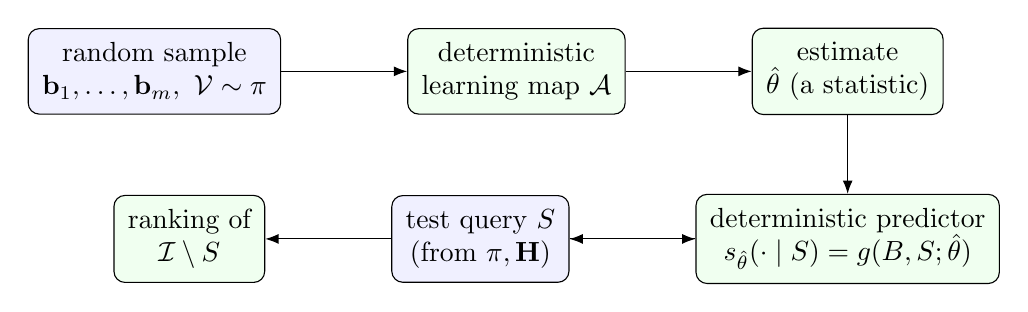
\begin{tikzpicture}[
  node distance=8mm and 16mm,
  box/.style={draw,rounded corners,align=center,inner sep=5pt,minimum height=9mm},
  rnd/.style={box,fill=blue!6},
  det/.style={box,fill=green!6},
  >=Latex
]
\node[rnd] (data) {random sample\\$\mathbf b_1,\dots,\mathbf b_m,\ \mathcal V \sim \pi$};
\node[det,right=of data] (A) {deterministic\\learning map $\mathcal A$};
\node[det,right=of A] (theta) {estimate\\$\hat\theta$ (a statistic)};
\node[det,below=10mm of theta] (g) {deterministic predictor\\$s_{\hat\theta}(\cdot\mid S)=g(B,S;\hat\theta)$};
\node[rnd,left=of g] (query) {test query $S$\\(from $\pi,\mathbf H$)};
\node[det,left=of query] (rank) {ranking of\\$\I\setminus S$};
\draw[->] (data) -- (A);
\draw[->] (A) -- (theta);
\draw[->] (theta) -- (g);
\draw[->] (query) -- (g);
\draw[->] (g) -- (query);
\draw[->] (query) -- (rank);
\end{tikzpicture}
\end{center}
\noindent\textcolor{blue!60!black}{\textbf{Blue}} = stochastic (data process); \textcolor{green!50!black}{\textbf{green}} = deterministic (maps).

\paragraph{The verdict.}
\begin{itemize}
  \item \textbf{Randomness lives only in the data}: the law $\pi$, the mask $\mathbf H$, and the i.i.d.\ sampling.
  It defines the population objective $\RK$ \eqref{eq:poprisk} we estimate and makes $\hat\theta$ a random
  estimator.
  \item \textbf{The learning map $\mathcal A$ and the predictor $g$ are deterministic.} Given the data, the ranking
  of $\I\setminus S$ is a fixed (affine-linear-plus-$\arg\max$) function of $S$; batch invariance removes even
  implementation nondeterminism.
  \item \textbf{The one probability model inside the method (Normal--Normal EB) is posited and rejected}, so in
  practice $\hat\theta$ is an ERM point estimate and $s_{\hat\theta}$ a deterministic closed-form map.
\end{itemize}

\begin{center}
\fbox{\parbox{0.92\linewidth}{\centering
\textbf{In one sentence.} \textsc{BundleFuse} is a deterministic, closed-form (predominantly linear-operator)
predictor whose finitely many parameters are an empirical-risk estimate from an i.i.d.\ bundle-generating process;
it is ``stochastic'' only as a statistical \emph{estimator} targeting a population recall functional, not as a
sampler.}}
\end{center}

\end{document}
